\documentclass{article}
\usepackage[utf8]{inputenc}
\usepackage{listings}
\usepackage{multicol}
\usepackage{amsmath}
\usepackage{color}
\usepackage{graphicx}


\title{HyperLogLog: Analysis and implementation of an improved algorithm}
\author{Dequeker Chloé, Ziat Ghiles}
\date{February 2015}

\begin{document}

\maketitle
\clearpage

\tableofcontents
\clearpage

\section{Introduction}
In this paper, we present our implementation and analysis of a
caridnality esmation algorithm proposed by Stefan Heule, Marc
Nunkesser and Alexander Hall: \texttt{HyperLogLog++}. This algorithm
is itself an improvement of the \texttt{HyperLogLog} algorithm
proposed by Flajolet et. al.

\subsection{cardinality estimation problem}
Finding the number of distinct elements in a data set with duplicates
is a well-known problem which applies in many fields.

The naive solution to this problem is to examine for each element of
the data stream its belonging to a data structure $\mathcal{D}$. If
$\mathcal{D}$ does not contain the element we add it to the data
structure. At the end of the process, the cardinality of the data
stream is equal to the size of $\mathcal{D}$.

This solution gives the exact answer but it is easy to see that it
scales very badly as the size of the data stream grows.

In order to resolve this problem, several alogorithms have been
proposed. These include LinearCounting and HyperLogLog which are the two
bases of the studied alogorithm.
\section{LinearCounting and HyperLogLog}
\subsection{LinearCounting}
\subsection{HyperLogLog}
The approach of the HyperLogLog algorithm to approximate the
cardinalities of a multiset is completely different. It is based on
randomization using a hash function for each element of the
multiset. It then focuses on the maximum of the number of leading
zeros in each hash values. it is legitimate to expect that the more
items there will be, the more this value will be high.  To improve the
precision of this calculation, HyperLogLog uses the stochastic
averaging technique: Doing so, it splits the stream in $m$ substreams,
and perform the computation separately on each.

The result is then subjected to corrections:
\begin{itemize}
\item \emph{Small range correction :} As shown by simulation, for a
  cardinality smaller than $\frac{5}{2}$ of the number of substreams, non-linear
  distortions appear. For that range, LinearCounting is used.
\item \emph{Large range correction :} Due to the use of a 32 bit hash
  function, when the cardinality goes to $2^{32}$, the chances of hash
  collisions increases.
\end{itemize}

\section{HyperLogLog++}

\subsection{transition to 64 bits}
Using a 32-bits hash function restricts the area of efficiency of the
algorithm to the sets with less then $2^{32}$ distincts elements.
That's why an proposed improvement is to use a 64-bits hash function.
It does not significatively change the memory cost (it is
 onlys increased only by 1 bit per substream).

\subsection{Bias estimation and correction}
For a given configuration of the algorithm, the observed bias is only
dependant on the cardinality estimated. From this observation, we
implement a correction method: As shown in figure 1, the raw
estimation of HLL is distorted for small cardinalities. In order to
correct this error, we take measures of it for cardinalities between 0
and 100 000 (with a step of 500) and we store them into a file. From
now, the file will be loaded at the begining of the calculation. A
correction may then be calculated for the result using a linear
interpolation between the values registered and the raw estimations.

\begin{center}
\begin{figure}[h]
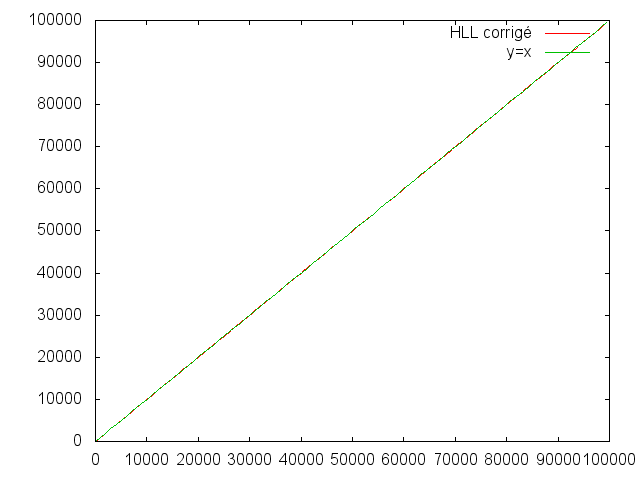
\includegraphics[scale=0.7]{img02.png}
\caption{Cardinality estimation for the corrected HLL}
\end{figure}
\end{center}


\subsection{Memory optimization}
\subsubsection{Sparse representation}
\subsubsection{Dense representation}
\subsubsection{Varint encoding}
Since the temporary set used in the sparse representation is merged
with the list before it gets too large, performing a compression on it
is not as interesting then on the sorted list. We'll try to reduce the
memory usage of it by playing on two points:
\begin{itemize}
\item Using fixed-size integers as it is common practice in many
  langages may here result in a waste of memory space.
\item Since the manipulated list is sorted, we can take advantage of
  this information.
\end{itemize}


\section{Conclusion}

\end{document}
